\section{Beschaffung der Daten}
\label{sec:data-mining}

Die Plattform \textit{Aviation Edge}\footnote{https://aviation-edge.com} stellt einige APIs und dahinterliegende Datenbanken
zur Verfügung, die Daten wie z.B. Standorte von Flughäfen sowie Routen von Airlines enthalten.
Die Daten können für einen Monatspreis von 5\$ (und später 99\$) abgerufen werden (Stand: Dezember 2018).
In den folgenden Unterabschnitten wird die Schnittstelle und das Datenformat kurz erläutert.

\subsection{Flughäfen}
\label{sec:airports}

Als Hauptknoten des zu untersuchenden Netzwerkes gelten die Flughäfen.
Diese können über die API über folgenden Aufruf der REST-Schnittstelle abgerufen werden:
\begin{lstlisting}
    GET https://aviation-edge.com/v2/public/airportDatabase?key=[API_KEY]
\end{lstlisting}
Die Serverantwort sieht wie folgt aus:

\begin{figure}[ht]
    \centering
    \begin{lstlisting}[language=json]
    [
        {
            "airportId": "1",
            "nameAirport": "Anaa",
            "codeIataAirport": "AAA",
            "codeIcaoAirport": "NTGA",
            "nameTranslations": "Anaa,Anaa,????,?????,????",
            "latitudeAirport": "-17.05",
            "longitudeAirport": "-145.41667",
            "geonameId": "6947726",
            "timezone": "Pacific/Tahiti",
            "GMT": "-10",
            "phone": "",
            "nameCountry": "French Polynesia",
            "codeIso2Country": "PF",
            "codeIataCity": "AAA"
        },
        ..
    ]

    \end{lstlisting}
    \caption{Inhalt der Server-Antwort der Airports-API}
    \label{lst:AirportsAPIResponse}
\end{figure}

Die API listet insgesamt 10050 Flughäfen.
Zum Vergleich bietet die Plattform \textit{ourairports.org} ebenfalls eine Liste mit weltweiten Flughäfen und -feldern an, enthält aber sogar
rund 50000 Einträge.
Nach einer ersten Einsicht in die Daten stellt sich allerdings heraus, dass die Vollständigkeit von Aviation Edge höher ist.
Für diese Arbeit wird deshalb und um die Komplexität möglichst gering zu halten auf die Verwendung dieses zusätzlichen Datensatzes verzichtet.

\subsection{Flugrouten}
\label{sec:routes}

Flugrouten von verschiedenen Fluggesellschaften können ebenfalls über \textit{Aviation-Edge} abgerufen werden.
Die Flugrouten repräsentieren im Netzwerk die Kanten zwischen den Knoten (Flughäfen).
Die API stellt die für den jeweiligen Tag gültigen bzw. registrierten Flugrouten bereit.
Über den folgenden Aufruf liefert die API die Routen:
\begin{lstlisting}
    GET https://aviation-edge.com/v2/public/routes?key=[API_KEY]&limit=1000000
\end{lstlisting}

Die API liefert standardmässig maximal 300 Einträge. Wird sie mit dem GET-Parameter \textit{limit} aufgerufen, kann
die Obergrenze auf ein beliebiges Limit gesetzt werden.
Die Grenze von einer Million reicht aus, um die insgesamt rund 208000 Einträge zu erhalten.
Die Daten haben die folgende Form:

\begin{figure}[ht]
    \centering
    \begin{lstlisting}[language=json]
    {
        "departureIata": "OTP",
        "departureIcao": "LROP",
        "departureTerminal": null,
        "departureTime": "09:15:00",
        "arrivalIata": "TRN",
        "arrivalIcao": "LIMF",
        "arrivalTerminal": null,
        "arrivalTime": "10:45:00",
        "airlineIata": "0B",
        "airlineIcao": "BMS",
        "flightNumber": "101",
        "regNumber": [
            "YR-BAP"
        ]
    }
    \end{lstlisting}
    \caption{Inhalt der Server-Antwort der Airports-API}
    \label{lst:routesAPIResponse}
\end{figure}

Für die Untersuchungen werden die Datensätze vom 8. Oktober 2018 (Flughäfen) bzw. vom 9. November 2018 (Flugverbindungen) verwendet.


\subsection{Datenaufbereitung}
\label{subsec:dataCleancing}

In ihrer Rohfassung bilden die erwähnten Datensätze kein Netzwerk.
In diesem Abschnitt wird kurz erläutert, wie die einzelnen Datensätze zu einem Netzwerk verbunden werden.
Dazu kommen die Python-Bibliothek \textit{NetworkX} sowie das Programm \textit{Gephi} zum Einsatz.

\subsubsection{Netzwerk-Dateiformat}
\label{subsec:networkFileformat}
Als nächstes müssen die Daten aus unterschiedlichen Quellen zu einem Netzwerk zusammengefügt werden.
Eines der Datenformate mit den meisten Features ist das GEXF\footnote{https://gephi.org/users/supported-graph-formats/}.
Die Spezifikation des Formats zeigt, dass es sich um ein herkömmliches XML-Format handelt\footnote{https://gephi.org/gexf/format/}.
Glücklicherweise bietet \textit{NetworkX} bereits Funktionen an, um das GEFX-Format zu lesen und zu schreiben\footnote{https://networkx.github.io/documentation/networkx-1.10/reference/generated/networkx.readwrite.gexf.write\_gexf.html}.


\subsubsection{Script zur Erstellung des Netzwerks}
Für das Kompilieren der Daten in das GEXF-Format wird ein Python-Script geschrieben.
Dafür wird der Gesamt-Graph erst mit networkX modelliert und anschliessend in das Format exportiert.
Das komplette Script ist auf Github einsehbar\footnote{https://github.com/samuelblattner/ffhs-na-semesterarbeit/blob/master/scripts/ffhs-na-semesterarbeit/generators/create\_airports\_network.py}.
Mit den beiden Funktionen \textit{load\_airports()} und \textit{load\_routes()} werden die beiden Roh-Datensätze geladen.
Anschliessend wird ein neues NetworkX-Netzwerk erstellt und sämtliche Flughäfen hinzugefügt.
Schliesslich werden all diejenigen Routen eingefügt, die einen Abflughafen und einen Ankunftsflughafen enthalten, die
dem Netzwerk bereits bekannt sind.

Ein weiteres wichtiges Detail anschliessend hinzugefügt: Die Abflug- sowie Ankunftszeit in Coordinated Universal Time (UTC).
Erst die normalisierten Abflug und Ankunftszeiten machen einen Vergleich und die Simulation der weltweiten Flugbewegungen möglich.


\subsubsection{Erste Betrachtung der Daten}
Ein erstes Laden des Netzwerks in Gephi und die Darstellung mit dem \guillemotleft Geo Layout \guillemotright zeigt
deutlich sichtbar die Umrisse der Kontinente (siehe Abb. \ref{fig:firstLoadGephi}).

\begin{figure}[h]
    \centering
    \subfigure[Flughäfen zeichnen die Kontinente\label{fig:firstLoadGephi}]{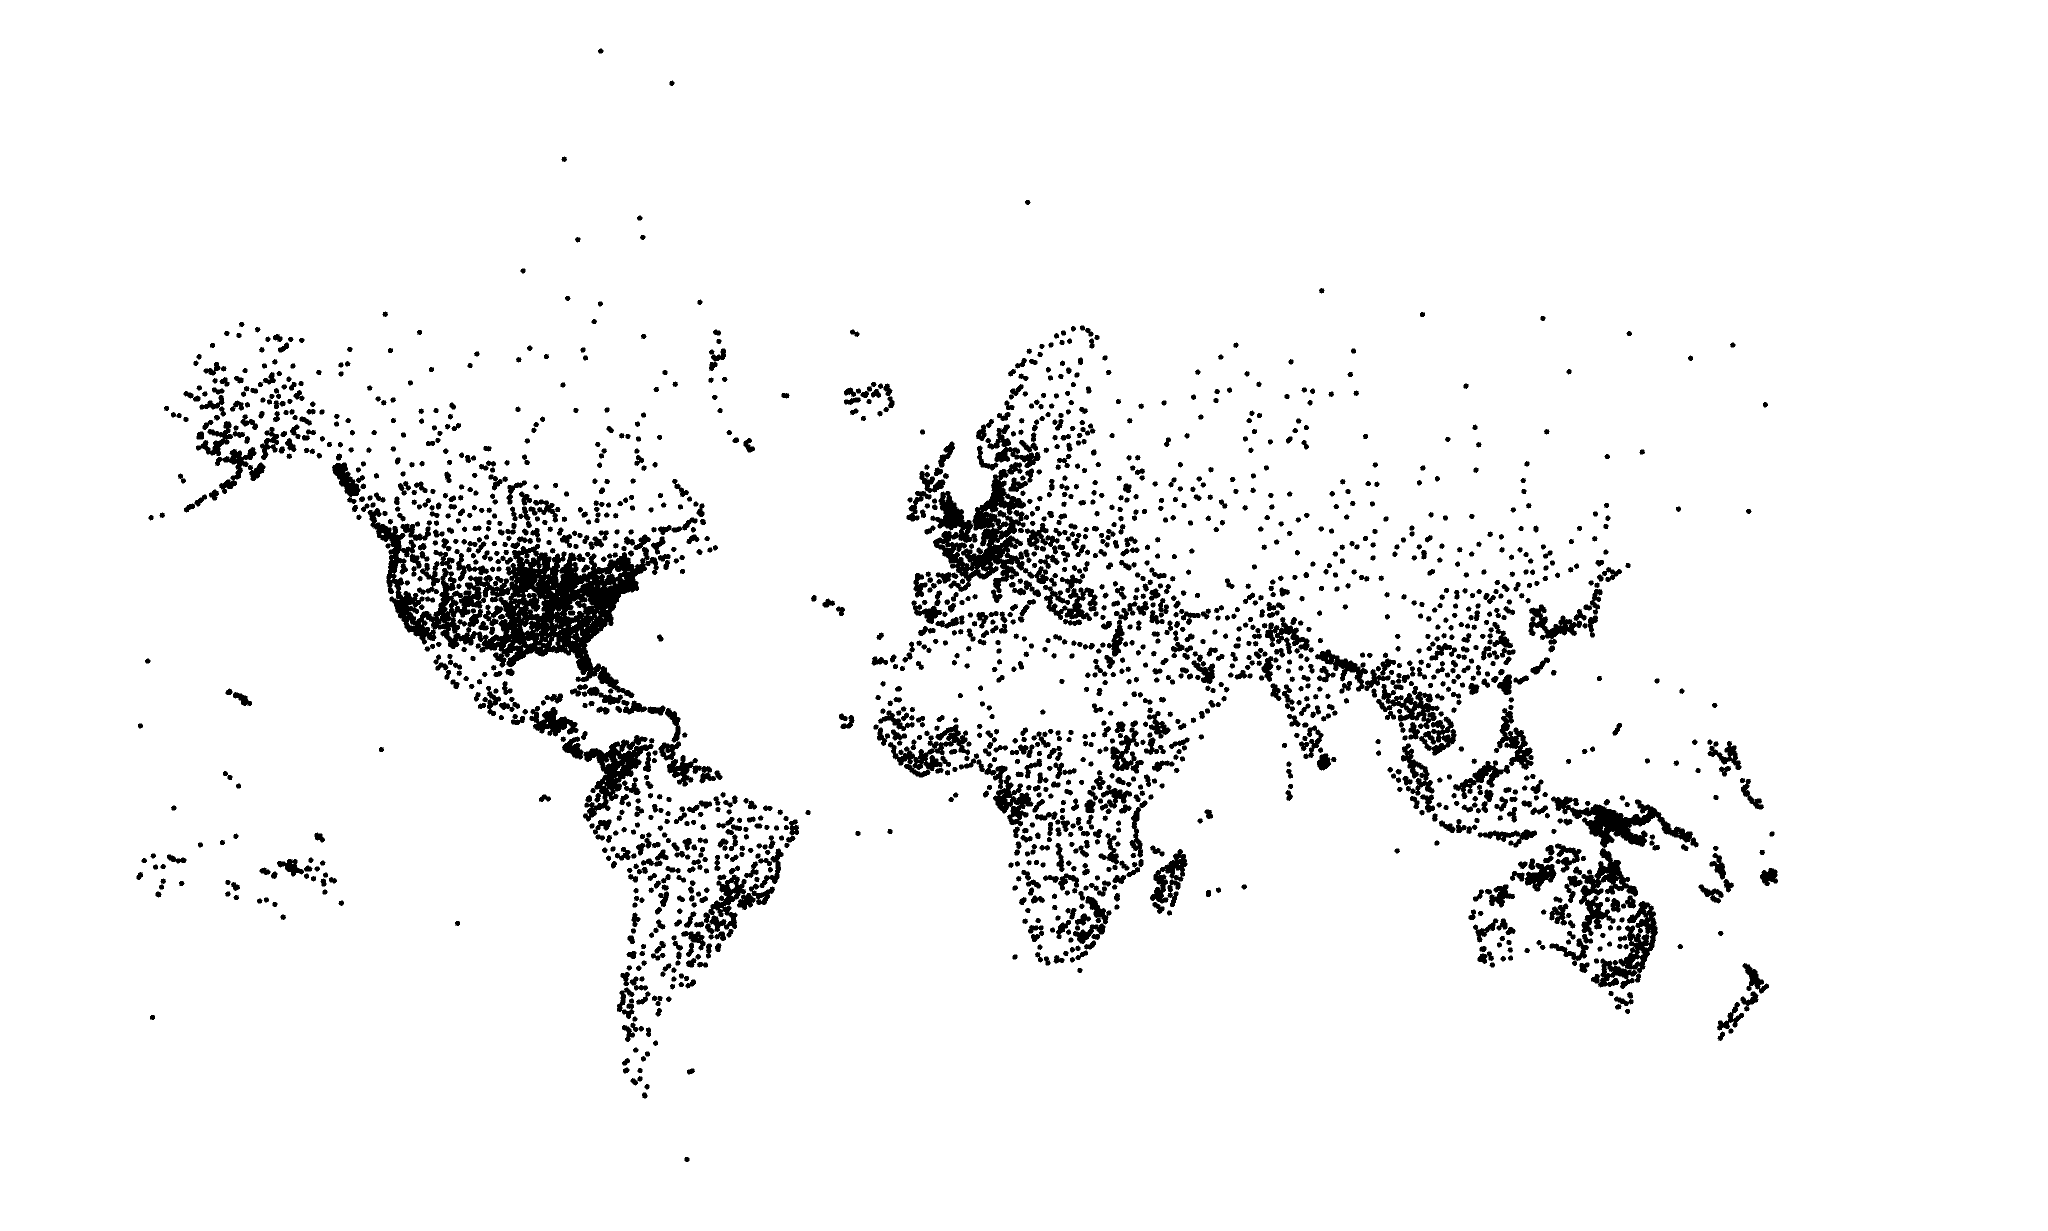
\includegraphics[width=\linewidth]{images/first-load-gephi.png}}
    \subfigure[Flugrouten geben erste Hinweise auf Cluster\label{fig:firstLoadGephiRoutes}]{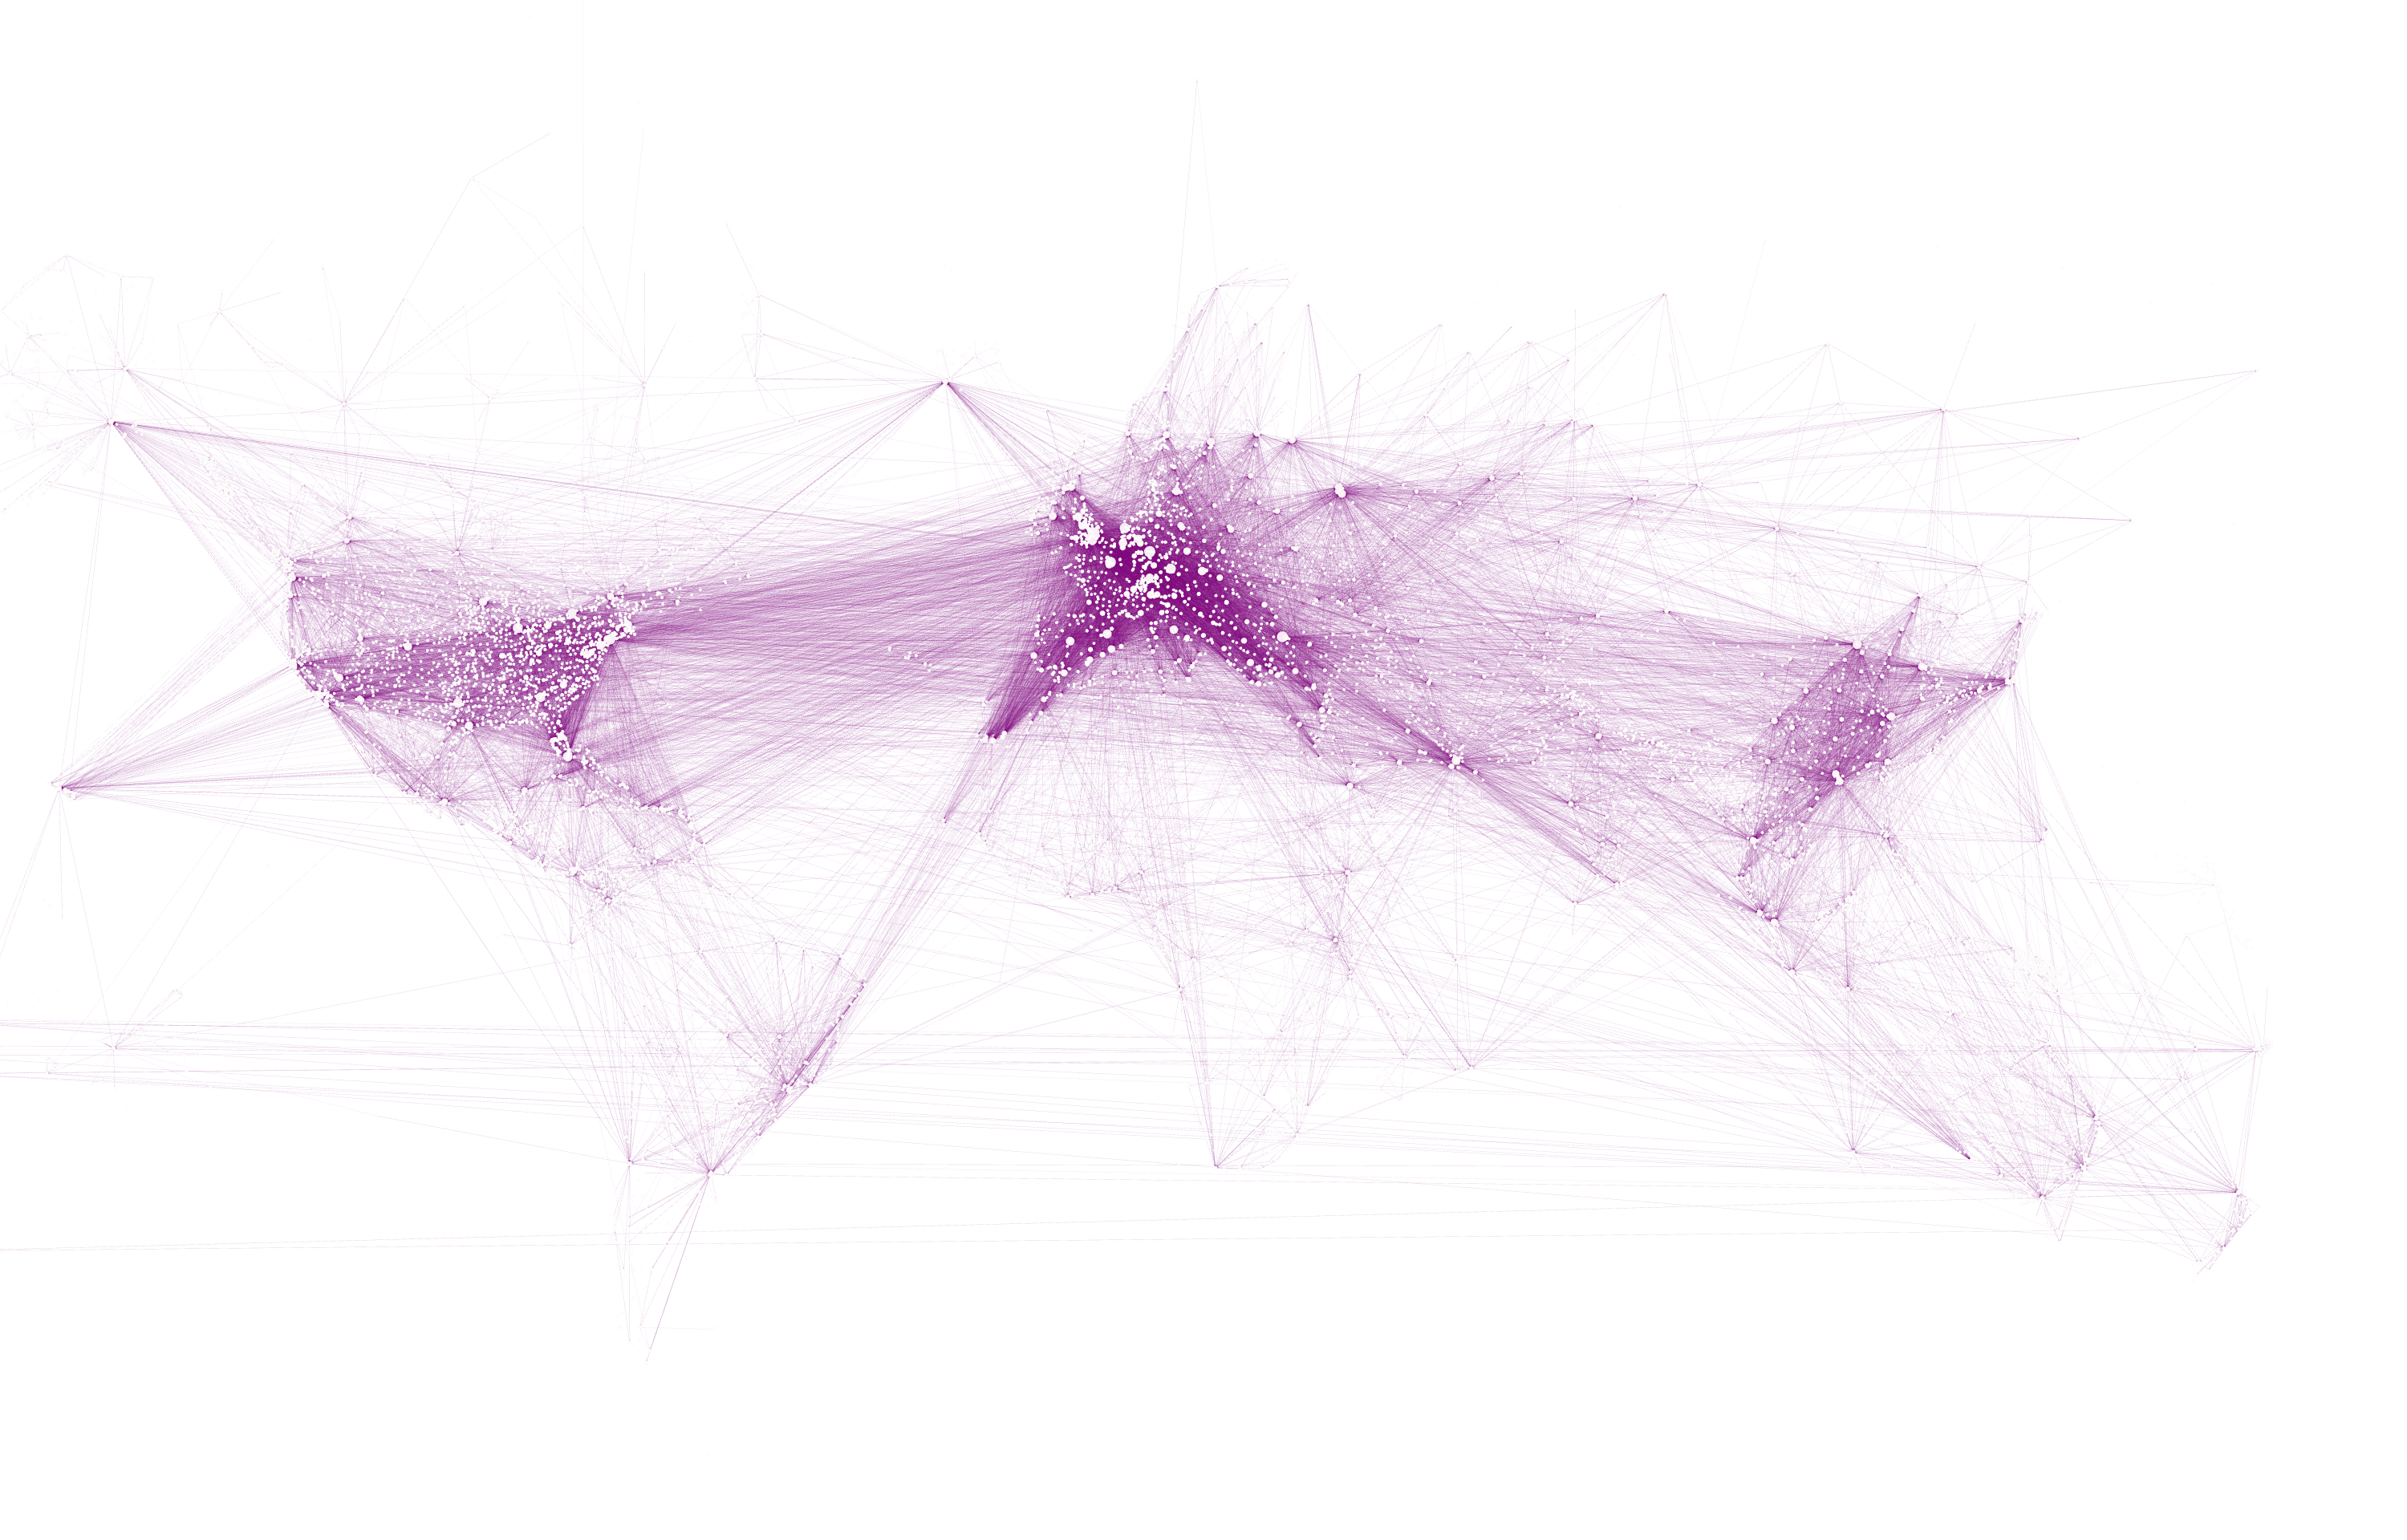
\includegraphics[width=\linewidth]{images/first-load-gephi-routes.png}}
\end{figure}

Werden die Routen dazugeladen ergibt sich das Bild in Abb. \ref{fig:firstLoadGephiRoutes}

Bei der ersten Überprüfung fällt auf, dass sich unter den Flughäfen einige Bahnhöfe verstecken.
Es ist nicht bekannt, weshalb diese Datensätze vorhanden sind.
Auch Aviation Edge schreibt nichts darüber.
Damit das Netzwerk möglichst nur Flughäfen und -felder enthält, werden die Bahnhöfe im Script entfernt.


